% use paper, or submit
% use 11 pt (preferred), 12 pt, or 10 pt only

\documentclass[letterpaper, preprint, paper,11pt]{AAS}	% for preprint proceedings
%\documentclass[letterpaper, paper,11pt]{AAS}		% for final proceedings (20-page limit)
%\documentclass[letterpaper, paper,12pt]{AAS}		% for final proceedings (20-page limit)
%\documentclass[letterpaper, paper,10pt]{AAS}		% for final proceedings (20-page limit)
%\documentclass[letterpaper, submit]{AAS}			% to submit to JAS

\usepackage{bm}
\usepackage{amsmath}
\usepackage{subfigure}
%\usepackage[notref,notcite]{showkeys}  % use this to temporarily show labels
\usepackage[colorlinks=true, pdfstartview=FitV, linkcolor=black, citecolor= black, urlcolor= black]{hyperref}
\usepackage{overcite}
\usepackage{footnpag}			      	% make footnote symbols restart on each page

% https://www.baen.com/rendezvous [1]


\PaperNumber{XX-XXX}



\begin{document}

%%% CHANGE TITLE SEE NOTES%%%%
\title{Rendezvous Proximity Operations Using Model Predictive Control with Dynamic Equations Derived Using SINDY and Dual Quaternions}

\author{Daniel Gonzalez\thanks{Title, department, affiliation, postal address.},
	 Mohammad Ayoubi\thanks{Title, department, affiliation, postal address.} , 
\ and Junette Hsin\thanks{Title, department, affiliation, postal address.}, 
}


\maketitle{} 		


\begin{abstract}
	
The abstract should briefly state the purpose of the manuscript, the problem to be addressed, the approach taken, and the nature of results or conclusions that can be expected. It should stand independently and tell enough about the manuscript to permit the reader to decide whether the subject is of specific interest. The abstract shall be typed single space, justified, centered, and with a column width of 4.5 inches. The abstract is not preceded by a heading of ``Abstract'' and its length may not extend beyond the first page.

\end{abstract}








\section{Introduction}
%Paper Title
%Rendezvous Proximity Operations Equations of Motion Derived with SINDy and Controlled with MPC
%
%Problem statement (general)

Space rendezvous missions have been extensively analyzed implementing various forms of constrained path planning and optimization techniques; many of which require high fidelity system identification of the chaser satellite. The combination of improvements in space-certified hardware and modern control techniques have expanded the capability of spacecraft control and the scope of on-orbit services. These advances have begun to democratize industry-changing missions like satellite refueling, inspection, and repair, along with debris removal or avoidance \cite{ParkZagaris_AnalysisandExperimention,cairano_park_MPC}. The increased need and application of these mission types has inspired further research in methods to lower costs, increase fuel savings, and find solutions to rendezvous problems with increasingly complex constraints, all while optimizing for computational efficiency.

One of those well-studied rendezvous methods utilizes model-predictive control (MPC), which has been shown to use less fuel due to minimum-fuel trajectory optimization while finding the best approach path within constraints of sensor visibility and safety. Richards and How developed and evaluated a new MPC implementation that optimizes using a novel mixed-integer linear programming method\cite{richards_how_MPC}. Fuel saving improvements over traditional MPC methods and the heritage glideslope approach. Singh and Bortolami presented an MPC solution to control one of the Space Shuttle's approach phases; they optimized for fuel and constrained the sensor line-of-sight and thruster firing directions to avoid plume impingement \cite{singh_bortolami_MPC}. They analyzed seven real-world cases of the space shuttle's standard orbit raising maneuver on its way to the ISS. Cairano and Park shows another example of how an MPC can be used for RPO maneuvers \cite{cairano_park_MPCApproach}. Their MPC implementation was robust to thrust errors, air drag (low Earth orbit), and solar pressure (geostationary orbits). They optimized considering time-to-dock and fuel consumption while constraining thrust magnitude, line-of-sight, and approach velocity. Kannan and Sajadi-Alamdari apply MPC to spacecraft rendezvous maneuvers while considering fuel-efficiency and collision avoidance in their cost function \cite{kannan_sajadi_MPC}. Park and Zagaris dive deeper into collision avoidance during rendezvous operations. Both linear and non-linear MPC methods are used to optimize fuel while avoiding obstacles, limit thrust magnitudes, and operating within safe entry cones. The linear technique uses hyperplanes to convexify obstacles while the nonlinear solution utilizes ellipsoids. The linear method proved to be much more robust, stable, and computationally practical.

Another control scheme that has been used for rendezvous maneuvers is called adaptive control. Filipe and Tsiotras proposed an adaptive position and attitude (pose) tracking controller for proximity operations that requires no knowledge about the mass and inertia of the chaser satellite \cite{filipe_tsiotras_dualQ}. It can also take into account gravitational acceleration, gravity-gradient torque, and other constant disturbance forces and torques. This method can perform system identification of the chaser satellite, given that sufficient conditions are met, and then proceed to approach and then dock the target satellite. 

For MPC, adaptive control, and other methods, offline and online system identification techniques are a necessity if high accuracy and precision control is desired, which many times requires costly and expensive volumes of data collection and processing. Within the previously cited adaptive control implementation, Filipe and Tsiotras calculate mass and inertia properties of the system by using known sets of disturbance forces and torques. With this method, the system identification is limited by the measurement quality of the applied forces and torques. There is another system identification technique that was investigated by Kaiser, Kutz, and Brunton that was used within an MPC method called sparse identification of nonlinear dynamics (SINDY) \cite{KaiserKutz_SparseID}. SINDY is a data-driven system identification algorithm which can be used to derive governing equations for a nonlinear dynamic systems. In this work, the authors compare SINDY to dynamic mode decomposition (DMD) and a multilayer neural network (NN). They show that sparse identification is preferred when a low volume of noisy data is available and a fast computation time is required. Also, SINDY sheds light on the underlying nonlinear dynamic equations of the system, instead of just having a black box that sheds little to no physical insight. Another strength of SINDY is that it is fast enough to run on embedded systems \cite{provost_williams_SINDY}. Lastly one of the most useful features of SINDY is that the system identification can be used in with control inputs along with other external forcing. SINDY has a few weaknesses, but they can be mitigated. The first is that a sufficient library of functions must be assumed to identify high-dimensional systems \cite{KaiserKutz_SparseID}; this can be prevented by increasing the function library size. Another drawback to this technique is that it does not react effectively to abrupt changes in dynamics, but this can be mitigated by using linear methods like DMD while the system dynamics settle\cite{KaiserKutz_SparseID}.
 

Robotics and spacecraft rendezvous operations go hand-in-hand, and the powerful tool known as dual quaternions, used mostly with robots, can brought over to bridge the gap to the on-orbit servicing realm \cite{valverde_tsiotras_spacecraftrobot}. This set of numbers extends the utility found in representing attitude as a quaternion to describe position or translation. Dual quaternions preferred over quaternion-vector representations for several reasons. Control laws can be written in a more compact form, pose transformations requires less computations than quaternion-vector method, natural coupling between rotational and translational motion is inherent, there is a strong parallel between rotational-only kinematics and rotation-translation dual quaternion kinematics, control stability is proven in one step, often controllers or filters developed for attitude quaternions can be adapted for use with dual quaternions, kinematics can be obtained easily because of multiplicative properties, constraint equations come in a simple form, and problems involving kinematic chains are more easily solved \cite{filipe_tsiotras_dualQ,tsiotras_valverde_DualQuatAsTool,dooley_mccarthy_spatialrigidbody}. Using this number set does come with what some may see as a drawback. Two additional constraint equations are necessary, derived motion relationships can be complicated, physical significance of variables are not initially apparent, and there is a quadratic cost on required control commands. \cite{dooley_mccarthy_spatialrigidbody,lee_mesbahi,constrainedautonomousprecision}


The contribution of this paper to the topics herein discuss
This paper will use SINDY for system identification within a model predictive controller for space rendezvous proximity operations (RPO). The improved efficiency from using dual quaternions over regular quaternions will be explored. 

\section{Dual Quaternion Concept Example}
All dynamics and controls equations discussed in this work are expressed using dual quaternions; before that is done, a quick introduction of this number set is given via an example. More thorough mathematical properties of quaternions, dual numbers, and dual quaternions are given in reference \citenum{filipe_tsiotras_dualQ}. Within the aerospace industry, single quaternions are used to express the attitude between two reference frames of interest. Combining quaternions with the concept of a dual number $\epsilon$, where $\epsilon^2 = 0$, but $\epsilon \ne 0$, allows the encoding of both rotational and translational information relating two reference frames. As an example, take the diagram in figure \ref{fig:Rel_Pos} showing the relative positions between chaser and target spacecraft orbiting a gravitational body. Using dual quaternions, one would express the pose of the chaser with respect to its target as
\begin{equation}
\begin{aligned}
\label{eq:dual_quat_eg}
\hat{q}_{B/D} = q_{B/D} + \epsilon \frac{1}{2} q_{B/D} r^B_{B/D},
\end{aligned}\\
\end{equation}
where $q_{B/D}$ represents the attitude unit quaternion and $r^B_{B/D}$ is the relative position vector represented as a quaternion. Using quaternion vector and scalar parts expressed in ordered pairs, the attitude is
\begin{equation}
\begin{aligned}
\label{eq:att_quat}
q_{B/D} = (\textbf{n}\sin{(\phi/2)} , \cos{(\phi/2)}) 
\end{aligned}\\
\end{equation}
where $\textbf{n}$ is the skew unit vector that one rotates frame D about by $\phi$ to get frame B. The relative position as a quaternion vector-scalar ordered pair is 
\begin{equation}
\begin{aligned}
\label{eq:pos_quat}
r_{B/D}^B = (\textbf{r}_{B/D}^B, 0).
\end{aligned}\\
\end{equation}


\begin{figure}[h!]
	\centering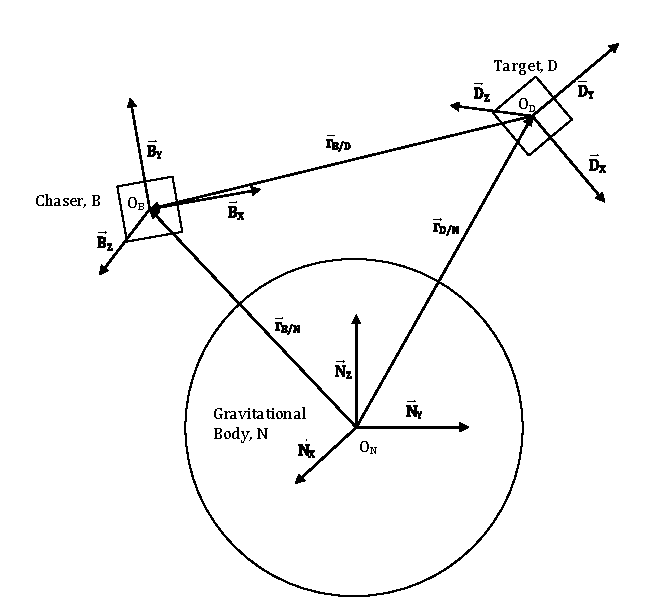
\includegraphics[width=3.5in]{Figures/REL_POSE.pdf}
	\caption{Relative positions between chaser and target spacecraft, orbiting a gravitational body.}
	\label{fig:Rel_Pos}
\end{figure}

\section{Relative Dynamic Equations for Rendezvous Proximity Operations}
Assuming quasi-static mass and inertial properties of a chaser spacecraft, B, its motion dynamics relative to a target body, D, are governed by
\begin{equation}
\begin{aligned}
	\label{eq:dyn}
	(\dot{\hat{\omega}}^B_{B/D})^s = (M^B)^{-1}\star(\hat{f}^B-(\hat{\omega}^B_{B/D}+\hat{\omega}^B_{D/N})\times(M^B\star((\hat{\omega}^B_{B/D})^s+(\hat{\omega}^B_{D/N})^s))\\-M^B\star(\hat{q}^*_{B/D}\dot{\hat{\omega}}^D_{D/N}\hat{q}_{B/D})^s-M^B\star(\hat{\omega}^B_{D/N}\times\hat{\omega}^B_{B/D})^s)
\end{aligned}\\
\end{equation}
where the dual inertia of the chaser is
\begin{equation}
\label{eq:dual_inertia}
M^B = 
\begin{bmatrix} 
mI_{3x3} & 0_{3x1} & 0_{3x3} & 0_{3x1} \\ 
0_{1x3} & 1 & 0_{1x3} & 0 \\ 
0_{3x3} & 0_{3x1} & \bar{I}^B & 0_{3x1} \\ 
0_{1x3} & 0 & 0_{1x3} & 1 
\end{bmatrix}, 
\end{equation}
given chaser mass $m$ and inertia in spacecraft fixed basis
\begin{equation}
\label{eq:sc_inertia}
\bar{I}^B = 
\begin{bmatrix} 
I_{11} & I_{12}& I_{13} \\ 
I_{21} & I_{22}& I_{23}\\ 
I_{31} & I_{32}& I_{33}
\end{bmatrix},
\end{equation}
and the total external dual force applied to the body about its mass center, in the spacecraft frame is
\begin{equation}
\label{eq:orbit_forces}
\hat{f}^B = \hat{f}^B_g + \hat{f}^B_{\nabla g} + \hat{f}^B_{J_2} +\hat{f}^B_{s}+\hat{f}^B_{\mu} + \hat{f}^B_d + \hat{f}^B_c.
\end{equation}
The components that make up the total external dual force, in the order shown in \eqref{eq:orbit_forces}, are gravitational acceleration, gravity-gradient torque, Earth-oblateness acceleration, solar dual force, atmospheric drag, dual disturbance force, and finally control dual force.

\section{SINDY With MPC}
This work will extend the application in reference \citenum{KaiserKutz_Sparse} to rendezvous maneuvers.
\begin{figure}[h!]
	\centering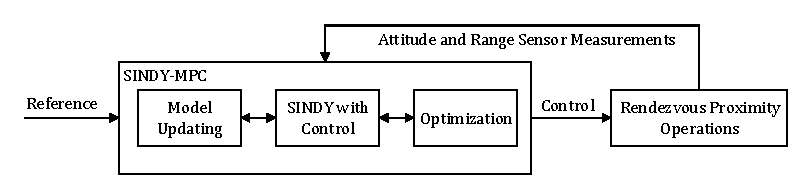
\includegraphics[width=3.5in]{Figures/SINDY_MPC.pdf}
	\caption{System identification using SINDY within model predictive control, for RPO.}
	\label{fig:SINDY_MPC}
\end{figure}
\begin{figure}[h!]
	\centering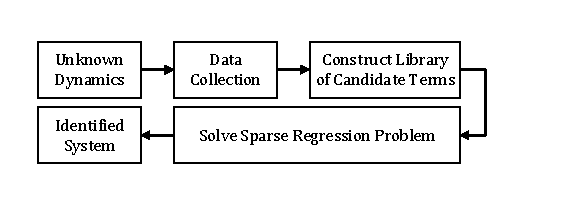
\includegraphics[width=3.5in]{Figures/SINDYC.pdf}
	\caption{Process of using measured data to identify nonlinear system dynamics.}
	\label{fig:SINCYC}
\end{figure}
%%% GUIDELINES
% The American Astronautical Society (AAS) publishes bound sets of printed conference proceedings for personal, institutional, and library usage. The availability of hardcopy enhances the longevity of your work and elevates the importance of your conference contribution to professionals through archival publication. To preserve the consistency and quality of the proceedings, all authors adhere to the latest version of AAS conference proceedings format.


% This document is intended to serve as a visual and instructional guide, and as a \LaTeX\ document template, for the AAS conference proceedings format. This template provides the basic font sizes, styles, and margins required by the publisher's formatting instructions.   There are also styles for centered equations, figure and table captions, section and sub-section headings, footnote text, \emph{etc}. This template provides samples of their usage.  To use this document as a template, simply copy and change its contents with your own information while maintaining the required predefined style, rather than starting anew. Since this is not a tutorial on how to use \LaTeX\, refer to \LaTeX\ manuals for more information.


% Your manuscript should include a paper number, a title, an author listing, an abstract, an introductory section, one or more sections containing the main body of the manuscript, a concluding summary section, and a reference or bibliography section. You may also include a section on notation, an acknowledgements section, and appendices, as illustrated in the sequel. You should \emph{not} include a leading cover sheet. Author affiliation shall appear on the first page, added as a footnote to the last name of each the author. If a distributional release statement or copyright notice is required by your sponsor, this is added as a footnote to the title of the manuscript, appearing on the first page only. Page numbers should be centered halfway between the lower margin and the bottom edge of the page (\emph{i.e.}, approximately 0.75 inches from the bottom). Copy should be single space with double space between paragraphs, with the first line of each paragraph indented 0.2 inches.

% The recommended sans-serif font for paper number, title, and author listing is \emph{Arial}, or, \emph{Helvetica}. The title font and paper-number font should be the same: 14-point sans-serif, centered, and bold. The author-listing font should be 12-point sans-serif, centered, and bold. The recommended serif font for body text, headings, \emph{etc}., is \emph{Times} or \emph{Times New Roman} at 10-12 point, 11 point preferred. The captions for figures and tables are bold 10-point serif font. The endnote reference text and footnote text is 9-point serif font. The right-hand margin of body text should be justified; if not, it should be fairly even nevertheless. All text and text background shall remain uncolored (black on white). These conventions should be automatically implemented in this \LaTeX\ template when the predefined styles of this template are used.

% The body text of this template is based on the preferred font size of 11 points. To change this to 12-point size, increase the font size at the top of the \LaTeX\ template by uncommenting the appropriate {\tt documentclass[]\{\}} line. For very long manuscripts, a 10-point font may be used to keep the manuscript within the publisher's limit of twenty (20) physical pages.



%%% NEEDS LOTS OF WORK 
%***
%
%Space rendezvous missions have been extensively analyzed using various forms of constrained path planning and optimization techniques. (REMOVE The ability to approach rendezvous missions with more stringent constraints has increased with the control capability.) The combination of sensor resolution and speed, modern control techniques along with faster processing, and finer actuation have made proximity operations more practical.
%
%(Make a better transition)A space rendezvous is a problem of performing orbit maneuvers where at least one active spacecraft and another, possibly passive space body converge onto the same orbit. Two classification groups are generally utilized when describing the spacecraft taking part in these types of missions: target and chaser. The goal in these rendezvous operations is to control the active chaser satellite with the objective to match its orbit velocity and position to that of the passive target body (should we place target and chaser in quotes?). Once the chaser gets sufficiently close to the target, it can hold its relative position constant, follow a profile about the objective, or approach the spacecraft for docking (We are assuming constant relative position REMOVE THIS).
%
%***
%
%*wordsmith* 
%Orbital rendezvous with a staellite in staitonary low-earth orbit has been extensively analyzed. Various forms of constrained path planning and optimization have been analyzed using modern optimization and serach techniques, however, as the capability and vaailability of targetting aids for cooperative proximity operations and docking have increased, the nature of the approach problem and the operational constraints during it have changed. 
%
%In this paper, we persent a new onboard optimal guidance and targetting approach using Model Predictive control, which explicitly incorporate sthe trajectory constraints associated with this transfer. A novel contribution of this approach is its ability to explicitly handle the trajectory state, control, and mission safety constraints. Model Predictive Control has been used in the process industries in chemical plants and oi lrefineries since the 1980s, but in the new millennium has found applications in the space engineering industry. The main advantage of MPC is the fact that is allows the current timeslot to be optimized, while keeping future timeslots into account. MPCs rely on dynamic models of hte process, most often linear empirical models obtained by system identification. 
%
%--> transition into SINDY
%*wordsmith* 
%
%Rendezvous proximity operations (RPO) are becoming more commonplace as they make servicing missions, etc (Look up what RPO can be used for) increasingly possible. A common challenge when planning an RPO mission is accurately determining, representing, and controlling the attitude, positions, and respective rates of the approaching spacecraft. A useful represention of the position and attitude measurements (pose) is dual . Use sensor data to approximate rendezvous proximity operations (RPO) equations of motion EOMs using SINDy. Implement model predictive control (MPC) with the approximated EOMs.
%
%CAUTION DO NOT PLAGIARIZE
%A space rendezvous is an orbital maneuver during which two spacecraft, one of which is often a space station, arrive at the same orbit and approach to a very close distance (e.g. within visual contact). Rendezvous requires a precise match of the orbital velocities and position vectors of the two spacecraft, allowing them to remain at a constant distance through orbital station-keeping. Rendezvous may or may not be followed by docking or berthing, procedures which bring the spacecraft into physical contact and create a link between them.
%
%The same rendezvous technique can be used for spacecraft "landing" on natural objects with a weak gravitational field, e.g. landing on one of the Martian moons would require the same matching of orbital velocities, followed by a "descent" that shares some similarities with docking.
%
%
%The standard technique for rendezvous and docking is to dock an active vehicle, the "chaser", with a passive "target". This technique has been used successfully for the Gemini, Apollo, Apollo/Soyuz, Salyut, Skylab, Mir, ISS, and Tiāngōng programs.[citation needed]
%
%To properly understand spacecraft rendezvous it is essential to understand the relation between spacecraft velocity and orbit. A spacecraft in a certain orbit cannot arbitrarily alter its velocity. Each orbit correlates to a certain orbital velocity. If the spacecraft fires thrusters and increases (or decreases) its velocity it will obtain a different orbit, one that correlates to the higher (or lower) velocity. For circular orbits, higher orbits have a lower orbital velocity. Lower orbits have a higher orbital velocity.
%
%For orbital rendezvous to occur, both spacecraft must be in the same orbital plane, and the phase of the orbit (the position of the spacecraft in the orbit) must be matched. The "chaser" is placed in a slightly lower orbit than the target. The lower the orbit, the higher the orbital velocity. The difference in orbital velocities of chaser and target is therefore such that the chaser is faster than the target, and catches up with it.[citation needed]
%
%Once the two spacecraft are sufficiently close, the chaser's orbit is synchronized with the target's orbit. That is, the chaser will be accelerated. This increase in velocity carries the chaser to a higher orbit. The increase in velocity is chosen such that the chaser approximately assumes the orbit of the target. Stepwise, the chaser closes in on the target, until proximity operations (see below) can be started. In the very final phase, the closure rate is reduced by use of the active vehicle's reaction control system. Docking typically occurs at a rate of 0.1 ft/s (0.030 m/s) to 0.2 ft/s (0.061 m/s).[16]
%CAUTION DO NOT PLAGIARIZE
%
%
%Related work
%Adaptive control with dual quaternions
%MPC with RPO and dual quaternions
%SINDy with control
%
%
%Advantage of our method
%
%
%
%One of the biggest challenges introduced
%by this technology is the need to simultaneously and accurately
%track both time-varying relative position and attitude references
%trajectories to avoid collisions between the satellites and achieve mission objectives.


%%% SPACE RENDEZVOUS DEFINITION 
%A space rendezvous is an orbit maneuver where two bodies in space converge onto the same orbit. Two classification groups are generally utilized when describing the spacecraft taking part in these types of missions: target and chaser. The goal in these rendezvous operations is to control the active chaser satellite to match the orbit velocity and position of the target body. Rendezvous operations can be broken down into two segments: inertial and relative. When the chase has the target outside of its sensor range, it is in the inertial segment of its approach. Once the chaser gets sufficiently close to reliably sense its target, it is in the relative segment of the approach, and proximity operations commence.  When in proximity operations it can: 
%
%1. hold its relative position constant, 
%2. follow a profile about the objective, 
%3. or approach the spacecraft for docking


%%% GUIDELINES 
%Numbering of section headings and paragraphs should be avoided. Major section headings are majuscule, bold, flush (aligned) left, and use the same style san-serif font as the body text. Widow and orphan lines should also be avoided; more than one line of a paragraph should appear at the end or beginning of a page, not one line by itself. A heading should not appear at the bottom of a page without at least two lines of text. Equations, figures, and tables must be sequentially numbered with no repeated numbers or gaps. Excessive white space --- such as large gaps before, between, and after text and figures --- should be minimal and eliminated where possible.


\subsection{This Is a Sample of a Secondary (Sub-Section) Heading}
%%% GUIDELINES 
%Secondary, or sub-section, headings are title case (miniscule lettering with the first letter of major words majuscule), flush left, and bold. Secondary headings use the same serif font style as the body text and, like section headings, should not be numbered. Tertiary headings should be avoided, but if necessary, they are run-in, italic, and end in a period, as illustrated with the next six (6) paragraphs.
%\begin{equation}
%	\label{eq:ab}
%	a = b^{2}
%\end{equation}

%\subsubsection{Equations.} 
%%% GUIDELINES
%Equations are centered with the equation number flush to the right. In the text, these equations should be referenced by name as Eq.~\eqref{eq:ab} or Equation~\eqref{eq:ab} (\emph{e.g}., not eq. 1, (1), or \emph{Equation 1}). To improve readability, scalar variable names such as $a$ and $b^{2}$ are usually italicized when appearing in text and equations.\footnote{A section on mathematical notation is provided in the sequel.}



%\subsubsection{Abbreviations.}
%%% GUIDELINES 
%When abbreviations for units of measure are used, lower case without periods is preferred in most instances; \emph{e.g}. ft, yd, sec, ft/sec, \emph{etc}., but in. for inch.
%
%
%
%
%\begin{figure}[htb]
%	\centering
\includegraphics[width=3.5in]{Figures/test}
%	\caption{Illustration Caption Goes Here}
%	\label{fig:xxx}
%\end{figure}

%\subsubsection{Figures.}   
%%% GUIDELINES
%Illustrations are referenced by name and without formatting embellishments, such as Figure~\ref{fig:xxx}, Figure 2, \emph{etc}., or, Figures 3 and 4 (\emph{e.g}., not figure (1), Fig. 1, \underline{Figure 1}, \emph{Figure 1}, \emph{etc}.). Each illustration should have a caption unless it is a mere sketch. Single-phrase captions are usually in title case; they are bold 10-point serif font and centered below the figure as shown in Figure~\ref{fig:xxx}. An explanatory caption of several sentences is permissible. Ideally, every illustration should be legibly sized -- usually about one-half or one-quarter page -- and appear in the text just before it is called out or mentioned. Alternatively, it is also permissible to place all figures together at the end of the text as a separate appendix; however, these two conventions should not be mixed. All figures and callouts should remain clearly legible after reduction. All illustrations appear as black and white in the final printing, although colors are retained in the electronic (CD-ROM) version.


\subsubsection{Graphic Formats.} 
%%% GUIDELINES
%The highest quality formats are Encapsulated PostScript (EPS) and PDF vector-graphic formats. These formats are recommended for all illustrations, unless they create document files that are excessively large. Specifically, you should change the graphic format or compress the image resolution whenever an illustrated page takes more than two seconds to render onscreen, or, whenever the total manuscript file size starts to approach 5 Mb. Photographs, illustrations that use heavy toner or ink (such as bar graphs), and figures without text callouts, may be suitably displayed with picture formats such as BMP, GIF, JPEG, PNG, TIFF, \emph{etc}. Line drawings, plots, and callouts on illustrations, should not use picture formats that do not provide sharp reproduction. All graphical content must be embedded when creating a PDF document, especially any fonts used within the illustration. Note that the Windows Metafile Format (WMF) is sometimes problematic and should be avoided.


\subsubsection{References and Citations.} 
%%% GUIDELINES
%The citation of bibliographical endnote references is indicated in the text by superscripted Arabic numerals, preferably at the end of a sentence.\cite{doe2005, style1959}   If this citation causes confusion in mathematics, or if a superscript is inappropriate for other reasons, this may be alternately expressed as (Reference~\citenum{doe2005}) or (see References~\citenum{doe2005} and \citenum{style1959}), (\emph{e.g}., not [1], Ref. (1), \emph{etc}.). While there is no singly prescribed format for every bibliographical endnote, references should be consistent in form. Citations should be sufficient to allow the reader to precisely find the information being cited, and should include specific pages, editions, and printing numbers where necessary. URL citations are discouraged, especially when an archival source for the same information is available. If a URL citation is required, it should appear completely and as a footnote instead of a bibliographical reference.\footnote{\url{http://www.univelt.com/FAQ.html\#SUBMISSION}}  The citation of private communication is especially discouraged, but if required it should be cited as a footnote and include the date, professional affiliation, and location of the person cited.\footnote{Gangster, Maurice (1999), personal correspondence of March 21st. Sr. Consultant, Space Cowboy Associates, Inc., Colorado Springs, CO.}  
%
%
%
%\begin{table}[htbp]
%	\fontsize{10}{10}\selectfont
%    \caption{A Caption Goes Here}
%   \label{tab:label}
%        \centering 
%   \begin{tabular}{c | r | r } % Column formatting, 
%      \hline 
%      Animal    & Description & Price (\$)\\
%      \hline 
%      Gnat      & per gram & 13.65 \\
%                & each     &  0.01 \\
%      Gnu       & stuffed  & 92.50 \\
%      Emu       & stuffed  & 33.33 \\
%      Armadillo & frozen   &  8.99 \\
%      \hline
%   \end{tabular}
%\end{table}
%
%\emph{Tables.} 
%Tables are referred to by name in the text as Table~\ref{tab:label}, or, Tables 2 and 3 (\emph{e.g}., not table 1, Tbl. 1, or \emph{Table 1}). The title is centered above the table, as shown in Table 1. The font size inside tables should be no larger than the body text, but may be adjusted down to 9-point if necessary (10-point serif font is considered nominal). Note that table units are in parentheses. Only the minimum number of table lines needed for clarity is desired. Ideally, every table should appear within the text just before it is called out, but, it is also permissible to place all tables together at the end of the text as a separate appendix. If so, these two conventions should not be mixed.
%
%Equations, figures, and tables must be sequentially numbered with no repeated numbers or gaps. Each figure and table shall be called out in the text; gratuitous figures and tables that are not called out should be eliminated. Intermediate equations may be numbered without being called out.




\section{Manuscript Submission}
%%% GUIDELINES
%The Portable Document Format (PDF) is the preferred format for electronic submissions.\footnote{By contributing your manuscript for proceedings publication, you necessarily extend any copyrights to the AAS and its designated publisher, to allow the AAS to publish your manuscript content in all the forms that it wishes.}
% The page size should be 8.5 inches by 11 inches exactly. You should use ``press-quality'' or ``high-quality'' software settings to create your PDF file; these settings tend to keep the PDF file true to the original manuscript layout, and automatically embed the correct fonts, \emph{etc}. Otherwise, settings such as ``Embed All Fonts'', \emph{etc}., should be selected as available. The use of internal hyperlinks within the electronic file is not encouraged because hyperlinks may not be supported in the final version of the electronic proceedings.

\subsection{Journal Submission}
%%% GUIDELINES
%If you wish to submit this manuscript to the \emph{Journal of Astronautical Sciences}, it must be re-formatted into a double-spaced format. This can be done easily with this template. At the top of the document, there are two (2) types document class statements ({\tt paper} and {\tt submit}).  The first type is the one to use for a conference paper.  The second type , which is commented out, can be used to reformat the paper for the JAS journal submission.


\section{Conclusion}
%%% GUIDELINES 
%Some AAS meetings are co-sponsored with the American Institute of Aeronautics and Astronautics (AIAA). When your paper number starts with ``AAS'', or when the conference is described as a joint ``AAS/AIAA'' meeting with the AAS listed first, this AAS conference proceedings format shall be used.
%
%Your final manuscript should be camera-ready as submitted --- free from technical, typographical, and formatting errors. Manuscripts not suitable for publication are omitted from the final proceedings.


\section{Acknowledgment}
%%% GUIDELINES 
%Any acknowledgments by the author may appear here. The acknowledgments section is optional.






\section{Notation}

%%% GUIDELINES 
%\begin{tabular}{r l}
%	$a$ & a real number \\
%	$b$ &  the square root of $a$ \\
%\end{tabular} \\

%If extensive use of mathematical symbols requires a table of notation, that table may appear here. Where the first mathematical symbol is introduced, a footnote should direct the attention of the reader to this table.\footnote{The footnote symbols are a standard sequence: $\ast$, $\dagger$, $\ddag$, \emph{etc}. This sequence of footnote symbols should restart with each new page.}  The notation table should be simple and reasonably consistent with the standards of modern technical journals, as illustrated above. The notation table does not need its own caption like an ordinary table, since the section heading serves this purpose. The notation section is optional.





\appendix
\section*{Appendix: Title here}
%%% GUIDELINES 
%Each appendix is its own section with its own section heading. The title of each appendix section is preceded by ``APPENDIX: '' as illustrated above, or ``APPENDIX A: '', ``APPENDIX B: '', \emph{etc}., when multiple appendixes are necessary. Appendices are optional and normally go after references; however, appendices may go ahead of the references section whenever the word processor forces superscripted endnotes to the very end of the document. The contents of each appendix must be called out at least once in the body of the manuscript.


\subsection*{Miscellaneous Physical Dimensions}

%%% GUIDELINES
%The page size shall be the American standard of 8.5 inches by 11 inches (216 mm x 279 mm). Margins are as follows: Top -- 0.75 inch (19 mm); Bottom -- 1.5 inches (38 mm); Left -- 1.25 inches (32 mm); Right -- 1.25 inch (32 mm). The title of the manuscript starts one inch (25.4 mm) below the top margin. Column width is 6 inches (152.5 mm) and column length is 8.75 inches (222.5 mm). The abstract is 4.5 inches (114 mm) in width, centered, justified, 10 point normal (serif) font.


\bibliographystyle{AAS_publication}   % Number the references.
\bibliography{references}   % Use references.bib to resolve the labels.



\end{document}
